\paragraph{Real-world examples of corruptions}
A more interesting set of experiments was conducted on the image data that exhibits real corruptions that can happen in the lab due to the wrong settings of the microscopy image acquisition approach. The following data was provided: 
\begin{figure}[htb]
	\begin{center}
		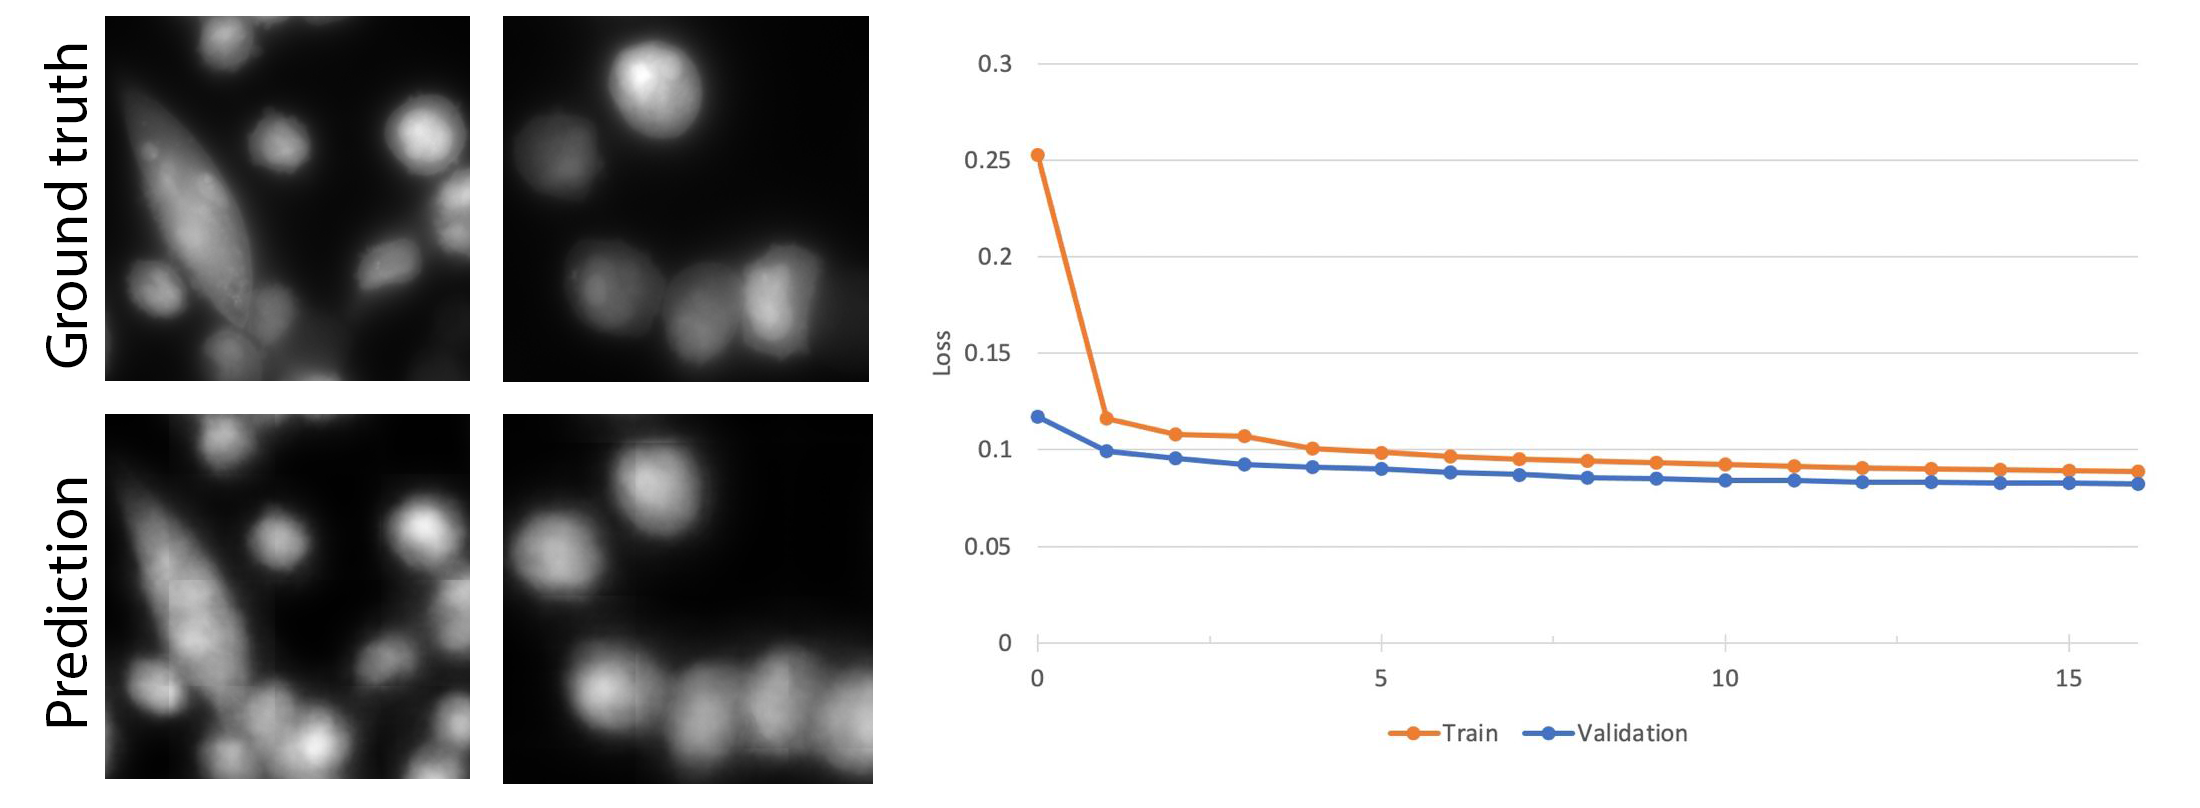
\includegraphics[width=\linewidth]{bilder/drift-detection/real corruptions/predictions.png}
		\caption{Real corrupted data from the lab}\label{fig:real-corruptions-predictions}
	\end{center}
\end{figure}


\begin{itemize}
    \item Figure \ref{fig:real-corruptions-predictions} (a) presents an example of the fixation of the cells in formalin for 15 minutes instead of the usual 10. These cells are more turbulent and more strongly clumped together. This is a good example of an image that cannot be simulated artificially with image processing.
    
    \item Figure \ref{fig:real-corruptions-predictions} (b) presents the same image with different microscope focus adjusments. From left to right: microscope stage lowered by 5 microns bringing the subject out of focus, normal height, higher microscope stage by 5 microns bringing the subject out of focus again but in the other direction.
    
    \item Figure \ref{fig:real-corruptions-predictions} (c) presents the same image with different exposure times. From left to right: 20ms --- underexposure, 30ms --- normal setting, 40ms --- overexposure.
\end{itemize}

The model tested here is the model trained on nucleus with simple augmentations (scale, rotation, flips). It seems that the time of formalin fixing does not really matter for nucleus outline, however the amount of details inside the nuclei seems to be slightly higher than with the usual fixation procedure. Focus of the microscope is clearly very important for good predictions. Although the negative direction of the focus loss seems to have better predictions than the positive one, many of the nuclei are simply gone in the fluorescence image in both cases. Over- and underexposure do not influence the predictions that drastically. Visually different exposure seems to change image brightness and the model is stable towards these changes. Nucleus outline stays mostly the same here as well, but the shining around it is dependent on the exposure times.